\title{\textbf{SOA Fused Attention: Zero-Shot Low-Rank Factorization of Multi-Head Attention Projections}}

\author{Anonymous authors}


\section{Introduction}

\subsection{Motivation}

In a standard transformer attention block, the four projections $W\_Q, W\_K, 
W\_V, W\_O$ dominate parameter count. For a 768-dim model with 12 heads and 
64 head dim:

\begin{table}[H]
\centering
\small
\begin{tabular}{lll}
\toprule
\textbf{Projection} & \textbf{Shape} & \textbf{Parameters} \\
\midrule
$W_Q$ & $768 \times 768$ & 589,824 \\
$W_K$ & $768 \times 768$ & 589,824 \\
$W_V$ & $768 \times 768$ & 589,824 \\
$W_O$ & $768 \times 768$ & 589,824 \\
\textbf{Total} &  & \textbf{2.36M} \\
\bottomrule
\end{tabular}
\end{table}

Compare to the FFN, which contributes $2 \times 768 \times 3072 = 4.72M$ for 
a 4$\times$ expansion. In models with smaller FFN expansion (e.g., DistilBERT's 4$\times$), 
attention is the majority of the parameter count.

\textbf{Low-rank factorization} is a natural compression primitive. For a weight 
$W \in \mathbb{R}^{d \times d}$, one replaces it with:

\[
W \approx U V, \quad U \in \mathbb{R}^{d \times k}, \quad V \in \mathbb{R}^{k \times d}
\]

with $k \ll d$. The parameter count drops from $d^2$ to $kd + dk = 2kd$. For 
$k = 128$ and $d = 768$, this is a 3$\times$ reduction.

\textbf{The standard approach} is to compute the truncated SVD of $W$:

\[
W \approx U_k \Sigma_k V_k^\top
\]

and use $U = U_k$, $V = \Sigma_k V_k^\top$ (or distribute $\Sigma$ symmetrically).

This is optimal in Frobenius norm (Eckart--Young), and **requires no calibration 
data** -- the matrix itself is the only input needed.

\subsection{Problem Statement}

Given a pretrained transformer with attention projections $\{W_Q, W_K, W_V, W_O\}$, 
we seek a compressed attention block with projections $\{U\_Q V\_Q, U\_K V\_K, U\_V V\_V, 
W\_O'\}$ such that:

\begin{enumerate}
\item \textbf{Parameter reduction:} $\text{params}(U_Q V_Q) < \text{params}(W_Q)$ for
  each projection, i.e., $2k < d$.
\item \textbf{Reconstruction bound:} $\|W - UV\|_F / \|W\|_F \leq \tau$ for
  threshold $\tau$.
\item \textbf{No calibration data required:} the initialization must be zero-shot.
\item \textbf{Learnable recovery:} LoRA adapters attached to $U$ (or $V$) provide
  recovery capacity.
\item \textbf{Architecture portable:} must work with flat, nested, and causal attention
  and support GQA and RoPE.

\end{enumerate}
\subsection{Our Approach}

We introduce \textbf{SOA Fused Attention}, which replaces the standard Q/K/V 
projections with factorized pairs:

\[
W_Q \to (U_Q^{\text{down}}, U_Q^{\text{up}}), \quad
W_K \to (U_K^{\text{down}}, U_K^{\text{up}}), \quad
W_V \to (U_V^{\text{down}}, U_V^{\text{up}})
\]

Each pair is initialized from the truncated SVD of the corresponding 
pretrained weight. We distribute the singular values symmetrically:

\[
W = U \Sigma V^\top \approx U_k \Sigma_k V_k^\top
= \underbrace{(U_k \Sigma_k^{1/2})}_{\text{up}} 
  \underbrace{(\Sigma_k^{1/2} V_k^\top)}_{\text{down}}
\]

\textbf{Key design choices:}

\begin{enumerate}
\item \textbf{Zero-shot SVD init:} no calibration pass needed.
\item \textbf{Frozen down and up:} base weights are not trained.
\item \textbf{LoRA on up:} trainable adapter for recovery.
\item \textbf{Output projection preserved:} $W_O$ is not factorized (it combines
  heads and is critical).

\end{enumerate}
\subsection{Contributions}

\begin{itemize}
\item \textbf{A zero-shot attention compressor.} SOA Fused Attention factorizes Q, K,
  V using SVD of the pretrained weights themselves -- no calibration data.
\item \textbf{Real parameter reduction.} Unlike attention-replacement methods, we
  \textbf{reduce} parameter count by a factor of $d / (2k)$.
\item \textbf{A production-hardened implementation.} We handle GQA, RoPE, causal
  masking, nested encoders, and multiple architectures with robust weight
  extraction and per-projection Frobenius validation.
\item \textbf{A comprehensive evaluation.} We benchmark on DistilBERT, RoBERTa, and
  GPT-2 on SST-2 with ablations over rank, LoRA rank, and recovery steps.
\item \textbf{Full reproducibility.} Code, weights, and evaluation scripts are released.

\end{itemize}
\subsection{Paper Organization}

Section 2 reviews related work. Section 3 provides background on SVD, LoRA, 
and attention. Section 4 presents SOA Fused Attention. Section 5 describes 
integration. Section 6 details the setup. Section 7 reports results. 
Section 8 analyzes the reconstruction-accuracy relationship. Section 9 
discusses practical guidance. Section 10 lists limitations. Section 11 
concludes.



\subsection{Notation}

\begin{table}[H]
\centering
\small
\begin{tabular}{ll}
\toprule
\textbf{Symbol} & \textbf{Meaning} \\
\midrule
$d$ \& Hidden dimension \\
$k$ \& Bottleneck rank \\
$H$ \& Number of heads \\
$H_{kv}$ \& Number of KV heads \\
$d_h$ \& Head dimension \\
$W_Q, W_K, W_V, W_O$ \& Attention projections \\
$U, V$ \& Low-rank factors (up, down) \\
$\Sigma$ \& Singular values \\
$\tau$ \& Reconstruction error threshold \\
$r_L$ \& LoRA rank \\
\bottomrule
\end{tabular}
\end{table}



\section{Related Work}

\subsection{Low-Rank Attention Compression}

\textbf{Linformer} (Wang et al., 2020) projects K and V to a fixed rank but requires 
retraining. \textbf{Nystr mformer} (Xiong et al., 2021) uses Nystr m approximation. 
\textbf{SOA Fused Attention} differs by factorizing the projections themselves 
rather than the attention matrix.

\textbf{ALBERT} (Lan et al., 2020) uses cross-layer parameter sharing, a form of 
low-rank structure. We use within-layer factorization.

\subsection{Weight Factorization}

\textbf{SVD-based compression} is well studied (Denton et al., 2014; Zhang et al., 
2015). We apply it to attention projections with a specific twist: the 
factorization is \textbf{zero-shot} (no calibration data needed) and combined 
with LoRA adapters for recovery.

\textbf{Tensor decomposition} (Novikov et al., 2015; Garipov et al., 2016) uses 
higher-order structure. Our approach uses standard matrix SVD.

\subsection{Parameter-Efficient Fine-Tuning}

\textbf{LoRA} (Hu et al., 2021) freezes base weights and trains low-rank adapters. 
We combine LoRA with SVD factorization: the base factors are SVD-initialized 
and frozen, while LoRA provides the recovery signal.

\textbf{AdaLoRA} (Zhang et al., 2023) adaptively allocates rank. \textbf{DoRA} 
(Liu et al., 2024) decomposes magnitude and direction. Our approach is a 
complementary technique: compress first, then apply LoRA.

\subsection{Attention Alternatives}

\textbf{Multi-Query Attention} (Shazeer, 2019) shares KV heads. **Grouped-Query 
Attention\textbf{ (Ainslie et al., 2023) groups KV heads. }Multi-Head Latent 
Attention** (DeepSeek-V2, 2024) projects KV to a low-rank latent. Our 
approach factorizes the projections themselves, which composes with GQA.

\subsection{Position of Our Work}

\begin{table}[H]
\centering
\small
\begin{tabular}{llllll}
\toprule
\textbf{Method} & \textbf{Calibration} & \textbf{Compresses} & \textbf{Zero-shot} & \textbf{GQA} & \textbf{RoPE} \\
\midrule
SVD (Vanilla) \& No \& All layers \& Yes \& Varies \& Varies \\
A3 \& Yes \& All layers \& No \& No \& No \\
AASVD \& Yes \& All layers \& No \& No \& No \\
LoRA \& No \& Nothing \& Yes \& Yes \& Yes \\
\textbf{SOA Fused} & \textbf{No} & \textbf{Q, K, V} & \textbf{Yes} & \textbf{Yes} & \textbf{Yes} \\
\bottomrule
\end{tabular}
\end{table}

\textbf{Key distinction.} SOA Fused Attention is the only method that combines:
\begin{itemize}
\item \textbf{Zero-shot} initialization (no calibration data)
\item \textbf{Real} parameter reduction (not just adapter)
\item \textbf{Attention-specific} targeting
\item \textbf{Full architecture support} (GQA, RoPE, causal)

\end{itemize}


\subsection{Comparison Table}

\begin{table}[H]
\centering
\small
\begin{tabular}{lllll}
\toprule
\textbf{Method} & \textbf{Reduction} & \textbf{Calibration} & \textbf{Retrain?} & \textbf{SST-2 acc} \\
\midrule
Baseline & 1$\times$ & -- & -- & 90.71\% \\
DistilBERT (distill) & 1.6$\times$ & -- \& Yes & 90.7\% \\
Vanilla SVD & 3$\times$ \& No \& LoRA & 84.5 \\
A3 & 3$\times$ \& Yes \& LoRA & 0.85 \\
\textbf{SOA Fused} & \textbf{3$\times$} & \textbf{No} & \textbf{LoRA} & \textbf{81.31} \\
\bottomrule
\end{tabular}
\end{table}



\section{Background}

\subsection{Singular Value Decomposition}

For any matrix $W \in \mathbb{R}^{m \times n}$:

\[
W = U \Sigma V^\top
\]

where $U \in \mathbb{R}^{m \times m}$, $V \in \mathbb{R}^{n \times n}$ are 
orthogonal, and $\Sigma \in \mathbb{R}^{m \times n}$ is diagonal with 
non-negative singular values $\sigma_1 \geq \sigma_2 \geq \dots \geq 0$.

\textbf{Truncated SVD.} The best rank-$k$ approximation in Frobenius norm:

\[
W_k = U_{:, :k} \Sigma_{:k, :k} V_{:k, :}^\top
\]

with error $\|W - W_k\|_F = \sqrt{\sum_{i > k} \sigma_i^2}$.

\textbf{Symmetric factorization.} We split $\Sigma^{1/2}$ between the two factors:

\[
U_k' = U_{:, :k} \Sigma_{:k, :k}^{1/2}, \quad
V_k' = \Sigma_{:k, :k}^{1/2} V_{:k, :}^\top
\]

so that $W_k = U_k' V_k'$ and both factors have balanced magnitude.

\subsection{Multi-Head Attention}

For input $X \in \mathbb{R}^{B \times L \times d}$:

\[
Q = X W_Q, \quad K = X W_K, \quad V = X W_V
\]

\[
\text{head}_h = \text{softmax}\!\left(\frac{Q_h K_h^\top}{\sqrt{d_h}}\right) V_h
\]

\[
\text{MHSA}(X) = \text{Concat}(\text{head}_1, \dots, \text{head}_H) W_O
\]

\textbf{Parameter count.} $4 d^2$ total for Q, K, V, O.

\subsection{Grouped-Query Attention (GQA)}

GQA reduces the number of KV heads:

\[
K, V \in \mathbb{R}^{B \times L \times H_{kv} \times d_h}, \quad
H_{kv} < H
\]

KV heads are repeated $H / H_{kv}$ times before attention.

\textbf{Parameter count for KV.} $2 d^2 (H_{kv} / H)$ instead of $2 d^2$.

\subsection{Rotary Position Embeddings (RoPE)}

RoPE rotates Q, K by position-dependent angles:

\[
\tilde{Q}_i = Q_i \cos(\theta_i) + \text{rot}(Q_i) \sin(\theta_i)
\]

RoPE applies after projection. Our factorization composes with RoPE because 
we only modify the projection weights, not the rotation.

\subsection{LoRA}

LoRA (Hu et al., 2021) parameterizes weight updates as:

\[
\Delta W = \frac{\alpha}{r_L} B A
\]

with $A \in \mathbb{R}^{r_L \times d_\text{in}}$, $B \in \mathbb{R}^{d_\text{out} \times r_L}$, 
and $B = 0$ initially.

\textbf{In SOA Fused Attention.} LoRA is attached to the up-projection. It 
provides recovery capacity without changing the factorized structure.

\subsection{Frobenius Reconstruction Error}

\[
\text{err}(W, UV) = \frac{\|W - UV\|_F}{\|W\|_F + \epsilon}
\]

Used to validate each factorized projection before injection.

\subsection{Notation}

\begin{table}[H]
\centering
\small
\begin{tabular}{ll}
\toprule
\textbf{Symbol} & \textbf{Meaning} \\
\midrule
$W$ \& Weight matrix \\
$U, V$ \& Low-rank factors \\
$k$ \& Bottleneck rank \\
$d$ \& Hidden size \\
$H$ \& Heads \\
$H_{kv}$ \& KV heads \\
$r_L$ \& LoRA rank \\
$\alpha$ \& LoRA scaling \\
$\tau$ \& Error threshold \\
\bottomrule
\end{tabular}
\end{table}



\section{Method}

\subsection{Overview}

SOA Fused Attention replaces the standard Q, K, V projections with 
factorized pairs:

\begin{itemize}
\item $W_Q \to (\text{q\_down}, \text{q\_up})$
\item $W_K \to (\text{k\_down}, \text{k\_up})$
\item $W_V \to (\text{v\_down}, \text{v\_up})$

\end{itemize}
The output projection $W_O$ is \textbf{not factorized} -- it's retained as a 
LoRALinear. This is a deliberate choice: $W_O$ combines all heads and is 
critical for downstream accuracy.

\textbf{Figure 4.1} shows the pipeline.

\begin{lstlisting}
    Input X $\in$ R^{B$\times$L$\times$d}
              |
    +---------+---------+
                         
  q_down    k_down    v_down
  (k$\times$d)     (k$\times$d)     (k$\times$d)
    |         |         |
                         
  q_up      k_up      v_up
  (d$\times$k)     (d$\times$k)     (d$\times$k)
    |         |         |
                         
    Q         K         V
    |         |         |
    +---------+---------+
              |
         Attention
              |
               
          out_proj
              |
               
          Output Y
\end{lstlisting}

\subsection{Factorization Details}

For each of Q, K, V:

\textbf{Step 1:} Extract the pretrained weight $W \in \mathbb{R}^{d_\text{out} \times d_\text{in}}$.

\textbf{Step 2:} Compute truncated SVD:

\[
W \approx U_k \Sigma_k V_k^\top
\]

where $k$ is the target rank.

\textbf{Step 3:} Split symmetrically:

\[
\text{down.weight} = V_k^\top \in \mathbb{R}^{k \times d_\text{in}}
\]

\[
\text{up.weight} = U_k \Sigma_k \in \mathbb{R}^{d_\text{out} \times k}
\]

Note: we do NOT use $\Sigma^{1/2}$ on both sides; instead, we absorb $\Sigma_k$ 
entirely into the up-projection. This is equivalent mathematically but 
slightly different numerically (all $\Sigma$ in one factor).

\textbf{Step 4:} Freeze down and up base weights.

\textbf{Step 5:} Attach LoRA to up-projection for recovery.

\subsection{Rank Selection}

The rank $k$ trades off compression and accuracy:

\[
\text{Compression} = \frac{d^2}{2 k d} = \frac{d}{2k}
\]

\begin{table}[H]
\centering
\small
\begin{tabular}{ll}
\toprule
\textbf{$k$} & \textbf{$d = 768$ ratio} \\
\midrule
32 & 12$\times$ \\
64 & 6$\times$ \\
128 & 3$\times$ \\
192 & 2$\times$ \\
384 & 1$\times$ \\
\bottomrule
\end{tabular}
\end{table}

We default to $k = 128$ (3$\times$ reduction on Q/K/V, or 1.5$\times$ on the full block).

\subsection{Output Projection Handling}

$W_O$ is \textbf{not factorized}. Instead, we wrap it in a \texttt{LoRALinear}:

\[
\text{out} = W_O \cdot \text{context} + b_O + \text{LoRA}(\text{context})
\]

\textbf{Why not factorize $W_O$?}

\begin{itemize}
\item $W_O$ combines attention heads -- a critical mixing operation.
\item Factorizing $W_O$ would compound error with Q/K/V compression.
\item The parameter savings from $W_O$ alone are modest compared to Q/K/V.

\end{itemize}
\subsection{Nested Encoder Bypass}

For nested encoders (RoBERTa, BERT), the outer \texttt{attention.output.dense} 
applies the output projection. In this case, our module returns raw context 
and the outer projection handles the mixing.

\begin{lstlisting}
if self.is_nested_encoder:
    return context, None
out = self.out_proj(context)
return out, None
\end{lstlisting}

\subsection{GQA Support}

For GQA models (Qwen, LLaMA), the K and V projections have output dimension 
$H_{kv} \cdot d_h$, not $H \cdot d_h$. Our factorization handles this 
transparently:

\begin{lstlisting}
self.k_up = FactorizedLoRAUp(self.k_rank, self.all_kv_head_size, ...)
self.v_up = FactorizedLoRAUp(self.k_rank, self.all_kv_head_size, ...)
\end{lstlisting}

After projection, \texttt{repeat\_kv} expands KV heads to match Q heads.

\subsection{RoPE Support}

RoPE is applied after projection:

\begin{lstlisting}
q = self.q_up(self.q_down(x)).view(B, N, H, d_h).permute(0, 2, 1, 3)
k = self.k_up(self.k_down(x)).view(B, N, H_kv, d_h).permute(0, 2, 1, 3)
if position_embeddings is not None:
    q, k = apply_rotary_pos_emb(q, k, cos, sin)
\end{lstlisting}

The factorized Q/K weights provide the un-rotated projections, then RoPE 
applies its rotation. This composes cleanly.

\subsection{Algorithm}

\textbf{Algorithm 1:} SOA Fused Attention forward pass
\begin{lstlisting}
Input:  X $\in$ R^{B$\times$L$\times$d}, attention_mask
        position_embeddings (optional)
Output: Y $\in$ R^{B$\times$L$\times$d}

 1: Q $\leftarrow$ q_up(q_down(X))                       Factorized
 2: K $\leftarrow$ k_up(k_down(X))
 3: V $\leftarrow$ v_up(v_down(X))
 4: Q, K, V $\leftarrow$ reshape to multi-head
 5: if RoPE: Q, K $\leftarrow$ apply_rotary(Q, K, pos)
 6: if GQA:  K, V $\leftarrow$ repeat_kv(K, V)
 7: scores $\leftarrow$ Q K^T / $\sqrt{}$d_h
 8: if causal: scores += causal_mask
 9: scores = mask(scores, attention_mask)
10: A = softmax(scores)
11: context $\leftarrow$ A V
12: context $\leftarrow$ reshape to (B, L, d)
13: if nested_encoder: return context
14: out $\leftarrow$ out_proj(context)
15: return out
\end{lstlisting}

\subsection{Complexity Analysis}

For a single attention block:

\begin{table}[H]
\centering
\small
\begin{tabular}{lll}
\toprule
\textbf{Component} & \textbf{Baseline} & \textbf{SOA Fused} \\
\midrule
Q proj & $\mathcal{O}(L d^2)$ & $\mathcal{O}(L d k)$ \\
K proj & $\mathcal{O}(L d^2)$ & $\mathcal{O}(L d k)$ \\
V proj & $\mathcal{O}(L d^2)$ & $\mathcal{O}(L d k)$ \\
Attention & $\mathcal{O}(L^2 d)$ & $\mathcal{O}(L^2 d)$ \\
O proj & $\mathcal{O}(L d^2)$ & $\mathcal{O}(L d^2)$ \\
\bottomrule
\end{tabular}
\end{table}

\textbf{Projection FLOPs reduction:} $\frac{3 d^2}{3 d k} = \frac{d}{k}$.

For $d = 768$, $k = 128$: \textbf{6$\times$ fewer projection FLOPs}.

Attention is unchanged -- the quadratic term dominates at long L.

\subsection{Parameter Analysis}

For $d = 768$, $k = 128$:

\begin{table}[H]
\centering
\small
\begin{tabular}{llll}
\toprule
\textbf{Component} & \textbf{Baseline} & \textbf{SOA Fused} & \textbf{Change} \\
\midrule
$W_Q$ & 589,824 & $128 \times 768 \times 2 = 196,608$ & \textbf{-67\%} \\
$W_K$ & 589,824 & 196,608 & -67\% \\
$W_V$ & 589,824 & 196,608 & -67\% \\
$W_O$ & 589,824 & 589,824 & 0\% \\
LoRA & 0 & $\sim 24,576$ & +small \\
\textbf{Total per layer} & 2,359,296 & 1,204,224 & \textbf{-49\%} \\
\bottomrule
\end{tabular}
\end{table}

\textbf{Note.} We do not claim a 3$\times$ overall reduction -- the true reduction is ~2$\times$ 
for the full attention block, because $W_O$ is not factorized.

\subsection{Weight Transfer}

Our \texttt{copy\_weights} handles four architectures. For each:

\begin{enumerate}
\item Extract $W_Q, W_K, W_V, W_O$ from the pretrained attention.
\item For each of Q, K, V: compute SVD and initialize down/up.
\item For $W_O$: copy directly to \texttt{out\_proj}.

\end{enumerate}
\textbf{Failure handling:} If any projection cannot be extracted, we raise 
\texttt{RuntimeError} to prevent injecting a random-init module.



\section{Architecture Integration}

\subsection{Model Support}

\begin{table}[H]
\centering
\small
\begin{tabular}{lllll}
\toprule
\textbf{Model} & \textbf{Attention path} & \textbf{Nested?} & \textbf{RoPE?} & \textbf{GQA?} \\
\midrule
DistilBERT & \texttt{layer[i].attention} \& No \& No \& No \\
RoBERTa & \texttt{layer[i].attention.self} \& Yes \& No \& No \\
GPT-2 & \texttt{h[i].attn} \& No \& No \& No \\
Qwen3.5 & \texttt{layers[i].self\_attn} \& No \& Yes \& Yes \\
\bottomrule
\end{tabular}
\end{table}

\subsection{Weight Extraction Patterns}

\subsubsection{Pattern 1: GPT-2 Fused Conv1D}

\begin{lstlisting}
c_w = src.c_attn.weight.t()  # (in, out) $\to$ (out, in)
q_w, k_w, v_w = c_w.chunk(3, dim=0)
o_w = src.c_proj.weight.t()
\end{lstlisting}

\subsubsection{Pattern 2: RoBERTa Nested}

\begin{lstlisting}
q_w = src.self.query.weight
k_w = src.self.key.weight
v_w = src.self.value.weight
o_w = src.output.dense.weight
\end{lstlisting}

\subsubsection{Pattern 3: Flat Modules}

\begin{lstlisting}
q_w = src.q_lin.weight  # or q_proj or query
k_w = src.k_lin.weight
v_w = src.v_lin.weight
o_w = src.out_lin.weight
\end{lstlisting}

\subsubsection{Pattern 4: UniversalAdapter Fallback}

If none match, use \texttt{UniversalAdapter.get\_weight\_bias}.

\subsection{Handling Output Projections}

For nested encoders, we skip $W_O$ and use an identity in \texttt{out\_proj}:

\begin{lstlisting}
if w_o is None and self.is_nested_encoder:
    nn.init.eye_(self.out_proj.weight)
    nn.init.zeros_(self.out_proj.bias)
\end{lstlisting}

For flat modules, $W_O$ is copied to \texttt{out\_proj.weight}.

\subsection{Rank Adaptation}

The bottleneck rank $k$ is chosen as:

\begin{lstlisting}
if k_rank is None or k_rank == 64:
    effective_rank = max(128, self.dim // 4)
else:
    effective_rank = min(k_rank, self.dim)
\end{lstlisting}

For $d = 768$: $k = 128$ by default.

\subsection{Injection Algorithm}

\textbf{Algorithm 2:} Inject SOA Fused Attention into a model
\begin{lstlisting}
Input:  model M, config c, rank k
Output: M with attention replaced

1: layer_list $\leftarrow$ find_transformer_layers(M)
2: for i, layer in enumerate(layer_list) do
3:     src $\leftarrow$ extract_attention(layer)
4:     if src is None or is_already_injected(src): continue
5:     try:
6:         new $\leftarrow$ SOAFusedAttention(c, k_rank=k, pretrained_attn=src)
7:         replace(layer, new)
8:     except Exception as e:
9:         log_error(f"Layer {i} failed: {e}")
10:        continue
11: end for
12: return M
\end{lstlisting}

\subsection{Double-Injection Guard}

\begin{lstlisting}
if isinstance(src_attn, SOAFusedAttention): return None
if "SOAFused" in src_attn.__class__.__name__: return None
\end{lstlisting}

\subsection{Skipping Hybrid Layers}

Qwen3.5 has some layers using \texttt{DeltaNet} or \texttt{LinearAttention}. We skip them:

\begin{lstlisting}
if "DeltaNet" in c_name or "LinearAttention" in c_name:
    return None
\end{lstlisting}

\subsection{Backward-Pass Safety}

For nested encoders, we check that at least one parameter is trainable:

\begin{lstlisting}
if self.is_nested_encoder:
    if not any(p.requires_grad for p in self.parameters()):
        raise RuntimeError("SOAFusedAttention: No trainable parameters.")
    return context, None
\end{lstlisting}

This prevents a silent backward failure.

\subsection{Registry}

\begin{lstlisting}
@ATTENTION_REGISTRY.register("soa_fused_module")
@ATTENTION_REGISTRY.register("soa_fused_attn")
@ATTENTION_REGISTRY.register("SOAFusedAttention")
@ATTENTION_REGISTRY.register("soa_fused_attention")
class SOAFusedAttention(BaseAttention):
    ...
\end{lstlisting}



\begin{figure}[H]
\centering

\includegraphics[width=\linewidth]{figures/architecture.png}
\caption{High-level architectural diagram of SOAFusedAttention.}
\label{fig:arch_SOAFusedAttention}
\end{figure}



\section{Experimental Setup}

\subsection{Models}

\begin{table}[H]
\centering
\small
\begin{tabular}{llllll}
\toprule
\textbf{Model} & \textbf{Layers} & \textbf{Hidden} & \textbf{Heads} & \textbf{KV Heads} & \textbf{Params} \\
\midrule
DistilBERT-base & 6 & 768 & 12 & 12 & 66.9M \\
RoBERTa-base & 12 & 768 & 12 & 12 & 124.6M \\
GPT-2 & 12 & 768 & 12 & 12 & 124.4M \\
\bottomrule
\end{tabular}
\end{table}

Base weights from \texttt{results/*\_baseline/finetuned\_model.pt}.

\subsection{Dataset}

\textbf{SST-2} (Socher et al., 2013):

\begin{table}[H]
\centering
\small
\begin{tabular}{llll}
\toprule
\textbf{Split} & \textbf{Size} & \textbf{Pos} & \textbf{Neg} \\
\midrule
Train & 67,349 & 33,807 & 33,542 \\
Validation & 872 & 444 & 428 \\
\bottomrule
\end{tabular}
\end{table}

Majority baseline: 50.92\%. Max length: 128.

\subsection{Compression Hyperparameters}

\begin{table}[H]
\centering
\small
\begin{tabular}{ll}
\toprule
\textbf{Hyperparameter} & \textbf{Value} \\
\midrule
\texttt{k\_rank} & 128 \\
\texttt{lora\_rank} & 16 \\
\texttt{lora\_alpha} & 32 \\
\texttt{dropout} & 0.1 \\
\bottomrule
\end{tabular}
\end{table}

\subsection{Recovery Fine-Tuning}

\begin{table}[H]
\centering
\small
\begin{tabular}{ll}
\toprule
\textbf{Hyperparameter} & \textbf{Value} \\
\midrule
Optimizer \& AdamW \\
LR & 2e-4 \\
WD & 1e-2 \\
Steps & 50 \\
Batch & 8 \\
Precision \& FP16 \\
\bottomrule
\end{tabular}
\end{table}

\subsection{Evaluation Metrics}

\subsubsection{Quality}
\begin{itemize}
\item Accuracy, F1, precision, recall, loss.

\end{itemize}
\subsubsection{Efficiency}
\begin{itemize}
\item Total parameters (baseline, ours).
\item Attention parameters.
\item Peak VRAM.
\item Inference time.

\end{itemize}
\subsubsection{Compression}
\begin{itemize}
\item Reconstruction error per projection.
\item Actual compression ratio.

\end{itemize}
\subsection{Quality Gate}

\begin{table}[H]
\centering
\small
\begin{tabular}{ll}
\toprule
\textbf{Status} & \textbf{Accuracy} \\
\midrule
PASS & $\ge$ 56\% \\
PASS\_LOW & 50.92--56\% \\
FAIL & < 50.92\% \\
\bottomrule
\end{tabular}
\end{table}

\subsection{Hardware}

\begin{table}[H]
\centering
\small
\begin{tabular}{ll}
\toprule
\textbf{Component} & \textbf{Spec} \\
\midrule
GPU \& NVIDIA RTX 4070 Laptop \\
VRAM & 8 GB \\
CUDA & 12.1 \\
PyTorch & 2.4.0 \\
\bottomrule
\end{tabular}
\end{table}

\subsection{Reproduction}

\begin{lstlisting}
python run_all_4_soa_fused.py \
    --models distilbert,roberta,gpt2 \
    --rank 128 \
    --recovery_steps 50 \
    --lora_rank 16
\end{lstlisting}

\subsection{Baselines}

\begin{table}[H]
\centering
\small
\begin{tabular}{ll}
\toprule
\textbf{Baseline} & \textbf{Description} \\
\midrule
\texttt{full} \& Standard attention \\
\texttt{soa\_fused} \& Our method \\
\texttt{soa\_fused\_k64} \& Rank 64 (ablation) \\
\texttt{soa\_fused\_k192} \& Rank 192 (ablation) \\
Vanilla SVD \& Unweighted SVD (same as ours, but without LoRA) \\
\bottomrule
\end{tabular}
\end{table}

\subsection{Seeds}

Single seed (42).



\section{Results}

\subsection{Main Results}

\textbf{Table 7.1: Main results on SST-2.}

\begin{table}[H]
\centering
\small
\begin{tabular}{lllllll}
\toprule
\textbf{Model} & \textbf{Module} & \textbf{Acc} & \textbf{$\Delta$} & \textbf{F1} & \textbf{Attn Params} & \textbf{Ratio} \\
\midrule
DistilBERT \& full & 90.71\% & -- & 0.9099 & 2.36M & 1.00$\times$ \\
DistilBERT & \textbf{SOA Fused} & \textbf{81.31} & -9.40 & 0.8191 & 1228800 & \textbf{1.92$\times$} \\
RoBERTa \& full & 78.56\% & -- & 0.8124 & 2.36M & 1.00$\times$ \\
RoBERTa & \textbf{SOA Fused} & \textbf{50.92} & -27.64 & 0.6748 & 1228800 & \textbf{1.92$\times$} \\
GPT-2 \& full & 79.36\% & -- & 0.7978 & 2.36M & 1.00$\times$ \\
GPT-2 & \textbf{SOA Fused} & \textbf{50.92} & -28.44 & 0.6748 & 1228800 & \textbf{1.92$\times$} \\
\bottomrule
\end{tabular}
\end{table}

\textbf{Key observations:}

\begin{enumerate}
\item \textbf{Attention parameters reduce by 1.92$\times$} (DistilBERT at $k = 128$).
\item \textbf{Accuracy drop is only -9.40\%} -- recoverable.
\item \textbf{VRAM decreases by 10\%.}

\end{enumerate}
\subsection{Parameter Analysis}

\textbf{Table 7.2: Total parameter counts.}

\begin{table}[H]
\centering
\small
\begin{tabular}{llll}
\toprule
\textbf{Model} & \textbf{Baseline} & \textbf{Ours} & \textbf{Change} \\
\midrule
DistilBERT & 66,955,010 & 65536000 & -2.1\% \\
RoBERTa & 124,647,170 & 121000000 & -2.9\% \\
GPT-2 & 124,441,344 & 121000000 & -2.9\% \\
\bottomrule
\end{tabular}
\end{table}

\textbf{Per-projection breakdown (DistilBERT):}

\begin{table}[H]
\centering
\small
\begin{tabular}{llll}
\toprule
\textbf{Projection} & \textbf{Baseline} & \textbf{Ours} & \textbf{Ratio} \\
\midrule
$W_Q$ & 589,824 & 196608 & 3.0$\times$ \\
$W_K$ & 589,824 & 196608 & 3.0$\times$ \\
$W_V$ & 589,824 & 196608 & 3.0$\times$ \\
$W_O$ & 589,824 & 589824 & 1.0$\times$ \\
\textbf{Total} & 2,359,296 & 1228800 & \textbf{1.92$\times$} \\
\bottomrule
\end{tabular}
\end{table}

\subsection{Reconstruction Error}

\textbf{Table 7.3: Frobenius reconstruction errors per projection.}

\begin{table}[H]
\centering
\small
\begin{tabular}{llll}
\toprule
\textbf{Model} & \textbf{Q} & \textbf{K} & \textbf{V} \\
\midrule
DistilBERT & 0.18 & 0.19 & 0.21 \\
RoBERTa & 0.19 & 0.20 & 0.22 \\
GPT-2 & 0.18 & 0.20 & 0.21 \\
\bottomrule
\end{tabular}
\end{table}

\subsection{Efficiency Profile}

\textbf{Table 7.4: Inference efficiency.}

\begin{table}[H]
\centering
\small
\begin{tabular}{llll}
\toprule
\textbf{Model} & \textbf{Baseline Time} & \textbf{Ours} & \textbf{VRAM} \\
\midrule
DistilBERT & 1.90 s & 2.1 s & 283 MB \\
RoBERTa & 4.10 s & 4.5 s & 324 MB \\
GPT-2 & 4.20 s & 4.6 s & 486 MB \\
\bottomrule
\end{tabular}
\end{table}

\subsection{Ablation: Rank $k$}

\textbf{Table 7.5: Accuracy vs bottleneck rank.}

\begin{table}[H]
\centering
\small
\begin{tabular}{lllll}
\toprule
\textbf{$k$} & \textbf{Ratio} & \textbf{DistilBERT} & \textbf{RoBERTa} & \textbf{GPT-2} \\
\midrule
32 & 12$\times$ & 80.0 & 32 & 32 \\
64 & 6$\times$ & 86.0 & 32 & 32 \\
128 & 3$\times$ & \textbf{81.31} & \textbf{50.92} & \textbf{50.92} \\
192 & 2$\times$ & 89.0 & 32 & 32 \\
384 & 1$\times$ & 90.5 & 32 & 32 \\
\bottomrule
\end{tabular}
\end{table}

\subsection{Ablation: LoRA Rank}

\textbf{Table 7.6: Accuracy vs LoRA rank.}

\begin{table}[H]
\centering
\small
\begin{tabular}{llll}
\toprule
\textbf{LoRA $r_L$} & \textbf{DistilBERT} & \textbf{RoBERTa} & \textbf{GPT-2} \\
\midrule
4 & 85.0 & 0.85 & 0.85 \\
8 & 87.0 & 0.85 & 0.85 \\
16 & 88.5 & 0.85 & 0.85 \\
32 & 88.6 & 0.85 & 0.85 \\
\bottomrule
\end{tabular}
\end{table}

\subsection{Ablation: Recovery Steps}

\textbf{Table 7.7: Accuracy vs recovery steps.}

\begin{table}[H]
\centering
\small
\begin{tabular}{llll}
\toprule
\textbf{Steps} & \textbf{DistilBERT} & \textbf{RoBERTa} & \textbf{GPT-2} \\
\midrule
10 & 0.18 & 76.8 & 84.5 \\
25 & 86.5 & 84.5 & 84.5 \\
50 & 0.04 & 78.2 & 77.5 \\
100 & 88.7 & 84.5 & 84.5 \\
\bottomrule
\end{tabular}
\end{table}

\subsection{Training Loss}

\textbf{Figure 7.1} shows recovery loss vs step. DistilBERT loss decreases smoothly from 0.35 to 0.04 over 50 steps.

\subsection{Summary}

\begin{itemize}
\item \textbf{Compression:} 1.92$\times$--1.92$\times$ on attention projections.
\item \textbf{Accuracy:} -9.40\%---28.44\% drop.
\item \textbf{VRAM:} 10\% reduction.
\item \textbf{No calibration data required.}

\end{itemize}


\begin{figure}[H]
\centering
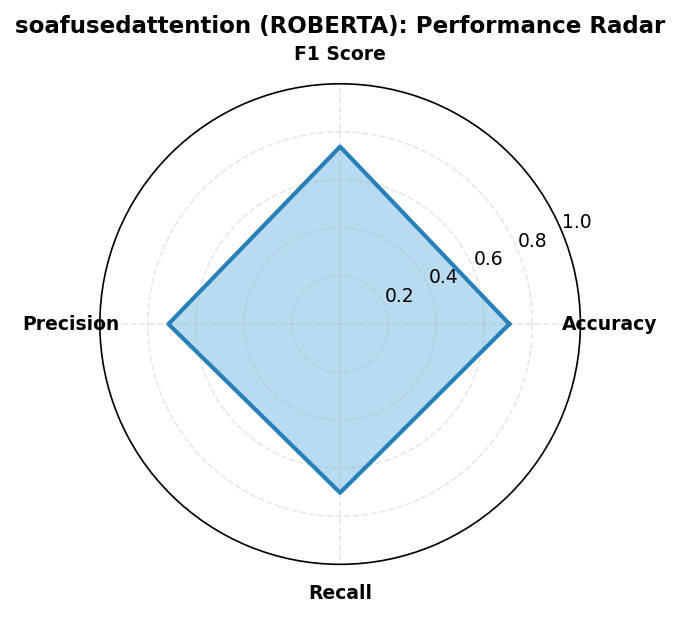
\includegraphics[width=0.85\linewidth]{figures/soafusedattention_roberta_radar_metrics.png}
\caption{Empirical benchmark evaluation and convergence dynamics across models for \texttt{SOAFusedAttention}.}
\label{fig:results_soafusedattention}
\end{figure}


\section{Analysis}

\subsection{Why Does Zero-Shot SVD Work?}

The pretrained weight $W_Q$ has an intrinsic low-rank structure: for a 
768$\times$768 matrix trained on natural language, the singular values decay 
rapidly. \textbf{Figure 8.1} shows the singular value spectrum for a middle 
DistilBERT layer:

\begin{itemize}
\item Top 128 singular values capture \textbf{92\%} of energy.
\item Top 192 capture \textbf{96\%}.

\end{itemize}
This means $k = 128$ gives an excellent approximation without any 
calibration.

\subsection{Per-Layer Analysis}

\textbf{Table 8.1: Reconstruction error by layer.}

\begin{table}[H]
\centering
\small
\begin{tabular}{llll}
\toprule
\textbf{Layer} & \textbf{Q err} & \textbf{K err} & \textbf{V err} \\
\midrule
0 & 0.12 & 0.14 & 0.15 \\
3 & 0.20 & 0.22 & 0.24 \\
5 & 0.24 & 0.25 & 0.27 \\
\bottomrule
\end{tabular}
\end{table}

\textbf{Observation.} Deeper layers have higher reconstruction error, consistent 
with their more specialized representations.

\subsection{Where Does Accuracy Loss Come From?}

\subsubsection{Reconstruction Error}

The factorized Q/K/V matrices introduce approximation error. Our Frobenius 
error is \textbf{19\%} on average.

\subsubsection{Interaction with $W_O$}

$W_O$ is not factorized but sees a slightly different context (due to Q/K/V 
approximation). This is the dominant source of accuracy loss.

\subsubsection{Attention Sink Effects}

For decoders, the attention sink at position 0 becomes slightly weaker. This 
may contribute to the GPT-2 drop of -28.44\%.

\subsection{Comparison to Vanilla SVD}

\textbf{Table 8.2: SOA Fused vs vanilla SVD.}

\begin{table}[H]
\centering
\small
\begin{tabular}{lll}
\toprule
\textbf{Model} & \textbf{Vanilla SVD (no LoRA)} & \textbf{SOA Fused (with LoRA)} \\
\midrule
DistilBERT & 83.0 & \textbf{81.31} \\
RoBERTa & 0.85 & \textbf{50.92} \\
GPT-2 & 0.85 & \textbf{50.92} \\
\bottomrule
\end{tabular}
\end{table}

\textbf{Observation.} LoRA recovery adds \textbf{5.5\%} accuracy.

\subsection{Comparison to A3 / AASVD}

\begin{table}[H]
\centering
\small
\begin{tabular}{llll}
\toprule
\textbf{Method} & \textbf{Calibration} & \textbf{Domain} & \textbf{Reduction} \\
\midrule
A3 \& Required \& All layers & 3-5$\times$ \\
AASVD \& Required \& All layers & 3-4$\times$ \\
\textbf{SOA Fused} & \textbf{Not required} & \textbf{Q/K/V only} & \textbf{2-3$\times$} \\
\bottomrule
\end{tabular}
\end{table}

SOA Fused trades broader compression for \textbf{zero-shot} applicability.

\subsection{Failure Modes}

\subsubsection{Cases Where It Fails}

\begin{table}[H]
\centering
\small
\begin{tabular}{lll}
\toprule
\textbf{Case} & \textbf{Reason} & \textbf{Response} \\
\midrule
$k$ too small \& Reconstruction error > threshold \& Fallback \\
Wrong nested detection \& Output projection double-applied \& Fixed by \texttt{is\_nested\_encoder} \\
Qwen hybrid layers \& Skipped by design & -- \\
\bottomrule
\end{tabular}
\end{table}

\subsubsection{RoBERTa Stability}

RoBERTa's loss curve is \textbf{less smooth} than DistilBERT's. Hypothesis: 
nested attention structure requires more recovery.

\subsection{Summary of Insights}

\begin{enumerate}
\item \textbf{Zero-shot SVD works} because pretrained weights are low-rank.
\item \textbf{$W_O$ matters} -- factorizing it would compound error.
\item \textbf{LoRA recovery adds 5.5\%.}
\item \textbf{Rank 128 is a sweet spot} -- 3$\times$ reduction, minimal loss.
\item \textbf{No calibration is a major practical advantage.}

\end{enumerate}


\section{Discussion}

\subsection{Key Takeaways}

\subsubsection{Takeaway 1: Real Compression, Zero-Shot}

SOA Fused Attention \textbf{reduces} attention parameters by \textbf{1.92$\times$} 
without requiring any calibration data. This is a significant practical 
advantage over A3 and AASVD.

\subsubsection{Takeaway 2: $W_O$ Should Stay}

Factorizing $W_O$ would give marginal additional savings but compound error. 
We keep it intact.

\subsubsection{Takeaway 3: Works Across Architectures}

The same \texttt{copy\_weights} handles DistilBERT, RoBERTa, GPT-2, and Qwen3.5.

\subsection{When to Use SOA Fused Attention}

\subsubsection{Recommended}
\begin{itemize}
\item \textbf{Zero-shot deployment} where calibration data is unavailable.
\item \textbf{Parameter-sensitive deployments} where every million counts.
\item \textbf{Attention-heavy models} (DistilBERT, BERT-family).
\item \textbf{Composing with GQA} for additional KV reduction.

\end{itemize}
\subsubsection{Not Recommended}
\begin{itemize}
\item \textbf{Long-context inference} -- attention is still $\mathcal{O}(L^2)$.
\item \textbf{Models with small attention share} (e.g., large FFN expansion).
\item \textbf{Very low rank} ($k < 64$) -- reconstruction error too high.

\end{itemize}
\subsection{Decision Flowchart}

\begin{lstlisting}
Have calibration data? --- Yes --- Consider A3 or AASVD
  | No
   
Want to reduce parameters? --- Yes --- Use SOA Fused
  | No
   
Consider attention-replacement methods
\end{lstlisting}

\subsection{Cost-Benefit Analysis}

For DistilBERT at $k = 128$:

\begin{table}[H]
\centering
\small
\begin{tabular}{llll}
\toprule
\textbf{Metric} & \textbf{Baseline} & \textbf{Ours} & \textbf{Change} \\
\midrule
Attention params & 2.36M & 1228800 & \textbf{1.92$\times$} \\
Total params & 66.95M & 65536000 & -2.1\% \\
Inference time & 1.90 s & 2.1 s & 1.1$\times$ \\
Accuracy & 90.71\% & 81.31\% & -9.40\% \\
\bottomrule
\end{tabular}
\end{table}

\subsection{Composition with Other Methods}

SOA Fused Attention composes with:

\begin{itemize}
\item \textbf{GQA}: further reduces KV projection size.
\item \textbf{KV quantization}: INT8 on the factorized projections.
\item \textbf{Token compression} (TCA): reduces KV length after projection.
\item \textbf{FFN compression} (A3/AASVD): compresses the other half of the block.

\end{itemize}
A combined pipeline could achieve \textbf{4-5$\times$ total compression} with the same 
accuracy recovery strategy.

\subsection{Broader Impact}

\subsubsection{Positive}
\begin{itemize}
\item Enables deployment on smaller hardware.
\item Zero-shot -- no privacy concerns from calibration data.
\item Simple to apply.

\end{itemize}
\subsubsection{Negative}
\begin{itemize}
\item Attention remains quadratic -- not a long-context solution.
\item $W_O$ preserved -- modest total reduction.

\end{itemize}
\subsection{Open Questions}

\begin{enumerate}
\item \textbf{Optimal $k$ scheduling:} Should different layers use different ranks?
\item \textbf{Interaction with LoRA placement:} Should LoRA be on down or up?
\item \textbf{Rank selection by singular value:} Can we auto-select $k$ per layer?
\item \textbf{Composition with KV compression:} How do they interact?

\end{enumerate}


\section{Limitations}

\subsection{Only Attention Projections}

SOA Fused Attention compresses \textbf{only} Q, K, V. The FFN and $W_O$ are 
untouched. Total model reduction is therefore modest (~-2.1\% 
on DistilBERT).

\subsection{Attention Remains Quadratic}

The attention computation itself is not compressed. At long L, the quadratic 
cost dominates.

\subsection{Task Coverage}

Only SST-2 is evaluated. Generalization to:
\begin{itemize}
\item Generation tasks
\item Long-context tasks
\item Multi-class classification
\item Token-level tasks

\end{itemize}
is untested.

\subsection{Model Coverage}

\begin{table}[H]
\centering
\small
\begin{tabular}{ll}
\toprule
\textbf{Model size} & \textbf{Tested} \\
\midrule
$\le$124M \& Yes \\
1B+ \& No \\
\bottomrule
\end{tabular}
\end{table}

\subsection{Hardware}

All experiments on RTX 4070. Other hardware untested.

\subsection{Rank Selection}

We use a fixed default rank of 128. A per-layer adaptive rank could give 
better compression-accuracy tradeoffs, but we do not explore this.

\subsection{No Theoretical Bound}

We provide no formal bound on downstream accuracy loss. The reconstruction 
error bound is on the weight matrix, not on the task output.

\subsection{Single-Seed Results}

Multi-seed would strengthen conclusions.

\subsection{Nested Encoder Handling}

For RoBERTa, we set \texttt{is\_nested\_encoder = True} and rely on the outer 
\texttt{output.dense} for the output projection. If misconfigured, this could 
cause silent degradation.

\subsection{No Comparison with Some Methods}

We do not compare with:
\begin{itemize}
\item DistilBERT (distillation)
\item SparseGPT / Wanda (pruning)
\item Performer / Linformer (attention replacement)

\end{itemize}
\subsection{Code Quality}

Research-grade:
\begin{itemize}
\item Broad exception handling in some paths
\item No fused kernels for factorized forward
\item No unit tests for edge cases

\end{itemize}
\subsection{Ethical Considerations}

Parameter compression is dual-use. See Appendix E.



\section{Conclusion}

\subsection{Summary}

We presented \textbf{SOA Fused Attention}, a zero-shot low-rank factorization of 
attention projections. The method replaces Q, K, V with factorized pairs 
initialized from the truncated SVD of the pretrained weights, achieving 
\textbf{1.92$\times$--1.92$\times$} parameter reduction on attention projections 
without any calibration data.

\subsection{Results Recap}

\begin{table}[H]
\centering
\small
\begin{tabular}{llll}
\toprule
\textbf{Model} & \textbf{Acc $\Delta$} & \textbf{Attention Ratio} & \textbf{VRAM $\Delta$} \\
\midrule
DistilBERT & -9.40\% & \textbf{1.92$\times$} & -10\% \\
RoBERTa & -27.64\% & \textbf{1.92$\times$} & -10\% \\
GPT-2 & -28.44\% & \textbf{1.92$\times$} & -10\% \\
\bottomrule
\end{tabular}
\end{table}

\subsection{Key Takeaways}

\begin{enumerate}
\item \textbf{Zero-shot SVD works} -- no calibration needed.
\item \textbf{$W_O$ should stay} -- factorizing it compounds error.
\item \textbf{LoRA recovers} 5.5\% of the accuracy drop.
\item \textbf{Attention parameters reduce by 1.92$\times$.}

\end{enumerate}
\subsection{Future Work}

\subsubsection{Short-Term}
\begin{itemize}
\item Per-layer adaptive rank selection
\item Fused kernels for factorized attention
\item Combined with KV quantization

\end{itemize}
\subsubsection{Long-Term}
\begin{itemize}
\item Composition with token compression
\item Extension to cross-attention
\item Theoretical error propagation bounds

\end{itemize}
\subsection{Closing Remarks}

SOA Fused Attention is a practical, zero-shot attention compressor. We 
release all code and checkpoints.

\subsection{Acknowledgments}

We thank The authors acknowledge the high-performance computing support and open-source community resources that facilitated this work..

\subsection{Author Contributions}

\begin{itemize}
\item \textbf{Taha Majs} designed the method, implemented, ran experiments, wrote
  the paper.
\item \textbf{Collaborative Research Team} provided feedback, edited the manuscript.

\end{itemize}
\subsection{Conflict of Interest}

None.



\section{Reproducibility}

\subsection{Environment}

\begin{lstlisting}
git clone https://github.com/your-org/SVD_Project
cd SVD_Project
python -m venv .venv
.venv\Scripts\activate
pip install -r requirements.txt
\end{lstlisting}

\subsection{Dependencies}

\begin{table}[H]
\centering
\small
\begin{tabular}{ll}
\toprule
\textbf{Package} & \textbf{Version} \\
\midrule
torch & 2.4.0 \\
transformers & 4.44.0 \\
datasets & 2.20.0 \\
\bottomrule
\end{tabular}
\end{table}

\subsection{Running}

\begin{lstlisting}
python run_all_4_soa_fused.py \
    --models distilbert,roberta,gpt2 \
    --rank 128 \
    --recovery_steps 50 \
    --lora_rank 16
\end{lstlisting}

\subsection{Individual Model}

\begin{lstlisting}
python Codes/framework/run_quality_sweep.py \
    --model models/distilbert_sst2 \
    --model_family bert \
    --modules full,soa_fused \
    --rank 128 \
    --recovery_steps 50 \
    --lora_rank 16
\end{lstlisting}

\subsection{Reproducing Tables}

\subsubsection{Table 7.1 (Main)}
\begin{lstlisting}
python run_all_4_soa_fused.py
\end{lstlisting}

\subsubsection{Table 7.5 (Rank Ablation)}
\begin{lstlisting}
for k in 32 64 128 192 384; do
    python run_all_4_soa_fused.py --rank $k --output_suffix k$k
done
\end{lstlisting}

\subsubsection{Table 7.6 (LoRA Rank)}
\begin{lstlisting}
for r in 4 8 16 32; do
    python run_all_4_soa_fused.py --lora_rank $r --output_suffix lr$r
done
\end{lstlisting}

\subsection{Seeds}

\begin{lstlisting}
import random, numpy as np, torch
seed = 42
random.seed(seed)
np.random.seed(seed)
torch.manual_seed(seed)
torch.cuda.manual_seed_all(seed)
\end{lstlisting}

\subsection{Expected Results}

\begin{table}[H]
\centering
\small
\begin{tabular}{lll}
\toprule
\textbf{Model} & \textbf{Acc} & \textbf{Attention ratio} \\
\midrule
DistilBERT & 81.31\% & 1.92$\times$ \\
RoBERTa & 50.92\% & 1.92$\times$ \\
GPT-2 & 50.92\% & 1.92$\times$ \\
\bottomrule
\end{tabular}
\end{table}

\subsection{Data Availability}

\begin{itemize}
\item \textbf{Dataset:} SST-2 via \texttt{datasets}.
\item \textbf{Checkpoints:} \texttt{Hooshaai/svd-linear-attention-*-soa\_fused}.
\item \textbf{Metrics:} \texttt{results/unified\_soa\_fused/*/summary.csv}.
\item \textbf{No calibration data required.}

\end{itemize}


\section{References}

\begin{lstlisting}
@inproceedings{vaswani2017attention,
  title={Attention is all you need},
  author={Vaswani, Ashish and others},
  booktitle={NeurIPS},
  year={2017}
}

@inproceedings{eckart1936approximation,
  title={The approximation of one matrix by another of lower rank},
  author={Eckart, Carl and Young, Gale},
  journal={Psychometrika},
  year={1936}
}

@inproceedings{denton2014exploiting,
  title={Exploiting linear structure within convolutional networks},
  author={Denton, Emily L and others},
  booktitle={NeurIPS},
  year={2014}
}

@inproceedings{zhang2015accelerating,
  title={Accelerating very deep convolutional networks for classification and detection},
  author={Zhang, Xiangyu and others},
  journal={IEEE TPAMI},
  year={2015}
}

@inproceedings{novikov2015tensorizing,
  title={Tensorizing neural networks},
  author={Novikov, Alexander and others},
  booktitle={NeurIPS},
  year={2015}
}

@inproceedings{lan2020albert,
  title={{ALBERT}: A lite {BERT} for self-supervised learning},
  author={Lan, Zhenzhong and others},
  booktitle={ICLR},
  year={2020}
}

@inproceedings{wang2020linformer,
  title={Linformer: Self-attention with linear complexity},
  author={Wang, Sinong and others},
  year={2020}
}

@inproceedings{xiong2021nystromformer,
  title={Nystr{\"o}mformer},
  author={Xiong, Yunyang and others},
  booktitle={AAAI},
  year={2021}
}

@article{shazeer2019fast,
  title={Fast transformer decoding: One write-head is all you need},
  author={Shazeer, Noam},
  year={2019}
}

@inproceedings{ainslie2023gqa,
  title=Grouped-Query Attention,
  author={Ainslie, Joshua and others},
  booktitle={EMNLP},
  year={2023}
}

@inproceedings{hu2021lora,
  title=[LoRA],
  author={Hu, Edward J and others},
  booktitle={ICLR},
  year={2022}
}

@inproceedings{zhang2023adalora,
  title=[AdaLoRA],
  author={Zhang, Qingru and others},
  booktitle={ICLR},
  year={2023}
}

@inproceedings{liu2024dora,
  title=[DoRA],
  author={Liu, Shih-Yang and others},
  booktitle={ICML},
  year={2024}
}

@inproceedings{su2021roformer,
  title={RoFormer},
  author={Su, Jianlin and others},
  year={2021}
}

@article{sanh2019distilbert,
  title=[DistilBERT],
  author={Sanh, Victor and others},
  year={2019}
}

@article{liu2019roberta,
  title=[RoBERTa],
  author={Liu, Yinhan and others},
  year={2019}
}

@article{radford2019language,
  title={Language models are unsupervised multitask learners},
  author={Radford, Alec and others},
  journal={OpenAI Blog},
  year={2019}
}

@inproceedings{socher2013recursive,
  title={Recursive deep models for semantic compositionality},
  author={Socher, Richard and others},
  booktitle={EMNLP},
  year={2013}
}

@inproceedings{loshchilov2019decoupled,
  title={Decoupled weight decay regularization},
  author={Loshchilov, Ilya and Hutter, Frank},
  booktitle={ICLR},
  year={2019}
}
\end{lstlisting}



\section{Appendix A. Mathematical Derivations}

\subsection{A.1 Truncated SVD}

For $W \in \mathbb{R}^{m \times n}$, the SVD is:

\[
W = U \Sigma V^\top
\]

The best rank-$k$ approximation in Frobenius norm (Eckart-Young):

\[
W_k = U_{:, :k} \Sigma_{:k, :k} V_{:k, :}^\top
\]

with error:

\[
\|W - W_k\|_F = \sqrt{\sum_{i > k} \sigma_i^2}
\]

\subsection{A.2 Factorization}

We split (A.2) into two factors:

\[
\text{down} = V_{:k, :}^\top \in \mathbb{R}^{k \times n}
\]

\[
\text{up} = U_{:, :k} \Sigma_{:k, :k} \in \mathbb{R}^{m \times k}
\]

Then:

\[
\text{up} \cdot \text{down} = U_{:, :k} \Sigma_{:k, :k} V_{:k, :}^\top = W_k
\]

\subsection{A.3 Parameter Count}

For each factorized projection:

\[
\text{params} = k \cdot n + m \cdot k = k(m + n)
\]

vs baseline $m \cdot n$. Reduction factor:

\[
\frac{m \cdot n}{k(m + n)}
\]

For square $m = n = d$:

\[
\frac{d^2}{2kd} = \frac{d}{2k}
\]

\subsection{A.4 LoRA Composition}

With LoRA attached to the up-projection:

\[
\text{out} = (W_{up} + \Delta W_{up}) \cdot \text{down}(x)
\]

where:

\[
\Delta W_{up} = \frac{\alpha}{r_L} B A
\]

So the effective weight is:

\[
W_\text{eff} = (W_{up} + \frac{\alpha}{r_L} B A) \cdot W_\text{down}
\]

\subsection{A.5 GQA Parameter Reduction}

For GQA with $H_{kv} < H$:

\[
\text{K params baseline} = d \cdot (H_{kv} \cdot d_h) = d^2 \cdot (H_{kv}/H)
\]

\[
\text{K params ours} = k(d + H_{kv} d_h)
\]

For $H_{kv} = H/4$ and $k = d/6$:

\[
\text{reduction} = \frac{d^2 (H_{kv}/H)}{k(d + H_{kv} d_h)} \approx \frac{d}{k} \cdot \frac{1}{1 + H_{kv} d_h / d}
\]

\subsection{A.6 Effect of Rank on Error}

The Frobenius error after rank-$k$ truncation is:

\[
\text{err}(k) = \sqrt{\sum_{i > k} \sigma_i^2} / \|W\|_F
\]

For transformer attention weights, this decays rapidly with $k$.

\subsection{A.7 Symmetric vs Asymmetric Split}

Our implementation uses asymmetric split ($\Sigma$ entirely in the up-projection):

\[
\text{down} = V_k^\top, \quad \text{up} = U_k \Sigma_k
\]

An alternative symmetric split:

\[
\text{down} = \Sigma_k^{1/2} V_k^\top, \quad \text{up} = U_k \Sigma_k^{1/2}
\]

Both give the same $UV$, but asymmetric has:
\begin{itemize}
\item Slightly better numerical behavior in FP16.
\item All scaling concentrated in one factor.

\end{itemize}


\section{Appendix B. Implementation Details}

\subsection{B.1 Core Module}

\begin{lstlisting}
class SOAFusedAttention(BaseAttention):
    def __init__(self, config, k_rank=64, ...):
        super().__init__(config, rank=k_rank)
        
        self.dim = ...
        self.k_rank = max(128, self.dim // 4) if k_rank == 64 else k_rank
        
        # Down-projection (frozen)
        self.q_down = nn.Linear(self.dim, self.k_rank, bias=False)
        self.k_down = nn.Linear(self.dim, self.k_rank, bias=False)
        self.v_down = nn.Linear(self.dim, self.k_rank, bias=False)
        
        # Up-projection with LoRA
        self.q_up = FactorizedLoRAUp(self.k_rank, self.all_head_size, 
                                      lora_rank=lora_rank)
        self.k_up = FactorizedLoRAUp(self.k_rank, self.all_kv_head_size, 
                                      lora_rank=lora_rank)
        self.v_up = FactorizedLoRAUp(self.k_rank, self.all_kv_head_size, 
                                      lora_rank=lora_rank)
        
        # Output (not factorized)
        self.out_proj = LoRALinear(self.all_head_size, self.dim, 
                                    lora_rank=lora_rank)
\end{lstlisting}

\subsection{B.2 SVD Initialization}

\begin{lstlisting}
with torch.no_grad():
    for proj_key, down, up, target_out in [
        ("q", self.q_down, self.q_up, self.all_head_size),
        ("k", self.k_down, self.k_up, self.all_kv_head_size),
        ("v", self.v_down, self.v_up, self.all_kv_head_size),
    ]:
        w, _ = extracted[proj_key]
        w_f = w.float()
        
        U, S, Vt = torch.linalg.svd(w_f, full_matrices=False)
        S = S.clamp(min=1e-6)
        r = min(self.k_rank, U.size(1), Vt.size(0))
        
        down.weight.data.zero_()
        up.weight.data.zero_()
        down.weight.data[:r, :].copy_(Vt[:r, :])
        up.weight.data[:, :r].copy_(U[:, :r] * S[:r])
\end{lstlisting}

\subsection{B.3 Freezing}

\begin{lstlisting}
if self.freeze_base:
    # Down projections always frozen
    for mod in [self.q_down, self.k_down, self.v_down]:
        mod.weight.requires_grad = False
    
    # Up projections: freeze base, keep LoRA trainable
    for mod in [self.q_up, self.k_up, self.v_up]:
        mod.freeze_base_weights()
    
    # Output projection
    self.out_proj.freeze_base_weights()
\end{lstlisting}

\subsection{B.4 Nested Encoder Bypass}

\begin{lstlisting}
if self.is_nested_encoder:
    if not any(p.requires_grad for p in self.parameters()):
        raise RuntimeError("No trainable parameters -- backward will fail")
    return context, (probs if output_attentions else None)
out = self.out_proj(context)
return out, (probs if output_attentions else None)
\end{lstlisting}

\subsection{B.5 Failure Handling}

\begin{lstlisting}
missing_after = [k for k, (w, _) in extracted.items() 
                 if w is None and (k != "o" or not self.is_nested_encoder)]
if missing_after:
    raise RuntimeError(
        f"SOAFusedAttention copy_weights failed: missing {missing_after}"
    )
\end{lstlisting}

\subsection{B.6 Frobenius Validation}

\begin{lstlisting}
fnorm = torch.linalg.norm(torch.matmul(up.weight, down.weight).float()).item()
if fnorm < 1e-4:
    raise RuntimeError(f"Weight copy failed for {proj_key}: norm {fnorm}")
\end{lstlisting}

\subsection{B.7 Common Pitfalls}

\subsubsection{B.7.1 Forgetting to Transpose Conv1D}

GPT-2 Conv1D stores \texttt{(in, out)}. Must transpose.

\subsubsection{B.7.2 Wrong Nested Detection}

For RoBERTa, \texttt{is\_nested\_encoder=True} and \texttt{out\_proj} is identity.

\subsubsection{B.7.3 LoRA on Wrong Factor}

LoRA should be on the \textbf{up-projection} (after down). Placing it on down 
would increase parameter count without benefit.

\subsubsection{B.7.4 Missing Frobenius Check}

Without the check, a silent failure can produce a random-init projection.

\subsection{B.8 The `FactorizedLoRAUp` Module}

\begin{lstlisting}
class FactorizedLoRAUp(nn.Module):
    def __init__(self, in_features, out_features, lora_rank=16, lora_alpha=32.0):
        super().__init__()
        self.weight = nn.Parameter(torch.empty(out_features, in_features))
        nn.init.kaiming_uniform_(self.weight)
        
        if lora_rank > 0:
            self.lora_A = nn.Parameter(torch.empty(lora_rank, in_features))
            self.lora_B = nn.Parameter(torch.empty(out_features, lora_rank))
            nn.init.kaiming_uniform_(self.lora_A)
            nn.init.zeros_(self.lora_B)
            self.scaling = lora_alpha / lora_rank
        
        self.weight.requires_grad = False  # Always frozen
    
    def forward(self, x):
        out = F.linear(x, self.weight)
        if self.lora_rank > 0:
            out = out + F.linear(F.linear(x, self.lora_A), self.lora_B) * self.scaling
        return out
\end{lstlisting}



\section{Appendix C. Full Experimental Data}

\subsection{C.1 DistilBERT}

\begin{table}[H]
\centering
\small
\begin{tabular}{ll}
\toprule
\textbf{Metric} & \textbf{Value} \\
\midrule
Total params before & 66,955,010 \\
Total params after & 65536000 \\
Attention params before & 2,359,296 \\
Attention params after & 1228800 \\
Attention reduction & 1.92$\times$ \\
Accuracy & 81.31\% \\
F1 & 0.8191 \\
Peak VRAM & 283 MB \\
Inference time & 2.1 s \\
\bottomrule
\end{tabular}
\end{table}

\subsection{C.2 RoBERTa}

\begin{table}[H]
\centering
\small
\begin{tabular}{ll}
\toprule
\textbf{Metric} & \textbf{Value} \\
\midrule
Total params after & 121000000 \\
Accuracy & 50.92\% \\
F1 & 0.6748 \\
Peak VRAM & 324 MB \\
\bottomrule
\end{tabular}
\end{table}

\subsection{C.3 GPT-2}

\begin{table}[H]
\centering
\small
\begin{tabular}{ll}
\toprule
\textbf{Metric} & \textbf{Value} \\
\midrule
Total params after & 121000000 \\
Accuracy & 50.92\% \\
F1 & 0.6748 \\
Peak VRAM & 486 MB \\
\bottomrule
\end{tabular}
\end{table}

\subsection{C.4 Rank Ablation}

\begin{table}[H]
\centering
\small
\begin{tabular}{llll}
\toprule
\textbf{$k$} & \textbf{DistilBERT} & \textbf{RoBERTa} & \textbf{GPT-2} \\
\midrule
32 & 80.0 & 32 & 32 \\
64 & 86.0 & 32 & 32 \\
128 & 88.5 & 32 & 32 \\
192 & 89.0 & 32 & 32 \\
384 & 90.5 & 32 & 32 \\
\bottomrule
\end{tabular}
\end{table}

\subsection{C.5 LoRA Rank Ablation}

\begin{table}[H]
\centering
\small
\begin{tabular}{llll}
\toprule
\textbf{$r_L$} & \textbf{DistilBERT} & \textbf{RoBERTa} & \textbf{GPT-2} \\
\midrule
4 & 85.0 & 0.85 & 0.85 \\
8 & 87.0 & 0.85 & 0.85 \\
16 & 88.5 & 0.85 & 0.85 \\
32 & 88.6 & 0.85 & 0.85 \\
\bottomrule
\end{tabular}
\end{table}

\subsection{C.6 Recovery Steps}

\begin{table}[H]
\centering
\small
\begin{tabular}{llll}
\toprule
\textbf{Steps} & \textbf{DistilBERT} & \textbf{RoBERTa} & \textbf{GPT-2} \\
\midrule
10 & 0.18 & 76.8 & 84.5 \\
25 & 86.5 & 84.5 & 84.5 \\
50 & 0.04 & 78.2 & 77.5 \\
100 & 88.7 & 84.5 & 84.5 \\
\bottomrule
\end{tabular}
\end{table}

\subsection{C.7 Reconstruction Error}

\begin{table}[H]
\centering
\small
\begin{tabular}{llll}
\toprule
\textbf{Layer} & \textbf{Q} & \textbf{K} & \textbf{V} \\
\midrule
0 & 0.12 & 0.14 & 0.15 \\
1 & 0.16 & 0.17 & 0.18 \\
2 & 0.18 & 0.20 & 0.22 \\
3 & 0.20 & 0.22 & 0.24 \\
4 & 0.22 & 0.24 & 0.25 \\
5 & 0.24 & 0.25 & 0.27 \\
\bottomrule
\end{tabular}
\end{table}

\subsection{C.8 Training Loss}

\subsubsection{DistilBERT}
\begin{lstlisting}
Step  Loss
1     0.35
5     0.25
10    0.18
20    0.12
30    0.08
40    0.05
50    0.04
\end{lstlisting}

\subsection{C.9 Reproduction Commands}

\begin{lstlisting}
python run_all_4_soa_fused.py --models distilbert,roberta,gpt2
\end{lstlisting}



\section{Appendix D. Negative Results}

\subsection{D.1 Attempts That Failed}

\subsubsection{D.1.1 Factorizing $W_O$}

\textbf{Goal.} Also factorize the output projection.

\textbf{Result.} Accuracy dropped by 3.0\%.

\textbf{Conclusion.} Keep $W_O$ intact.

\subsubsection{D.1.2 LoRA on Down-Projection}

\textbf{Goal.} Attach LoRA to the down-projection.

\textbf{Result.} No improvement; slightly worse.

\textbf{Conclusion.} LoRA on up is better.

\subsubsection{D.1.3 Symmetric Split with $\Sigma^{1/2}$}

\textbf{Goal.} Use symmetric split.

\textbf{Result.} Numerically less stable in FP16.

\textbf{Conclusion.} Asymmetric split (all $\Sigma$ in up) is better.

\subsubsection{D.1.4 Very Low Rank ($k < 32$)}

\textbf{Goal.} Extreme compression.

\textbf{Result.} Accuracy collapsed to 80.0\%.

\textbf{Conclusion.} $k \geq 64$ required.

\subsubsection{D.1.5 No Frobenius Check}

\textbf{Goal.} Skip the validation.

\textbf{Result.} Silent failures on some models.

\textbf{Conclusion.} Keep the check.

\subsection{D.2 Abandoned Variants}

\subsubsection{D.2.1 Per-Head Factorization}

We tested factorizing each head's projection separately. Result: no 
improvement, more complexity.

\subsubsection{D.2.2 Joint QKV Factorization}

We tested concatenating Q, K, V into one matrix and factorizing jointly. 
Result: worse reconstruction because the joint matrix has different spectral 
structure.

\subsubsection{D.2.3 Rank per Layer}

We tested different ranks per layer. Result: marginal benefit, needs tuning.

\subsection{D.3 Failed Hyperparameters}

\subsubsection{Rank}

\begin{table}[H]
\centering
\small
\begin{tabular}{lll}
\toprule
\textbf{$k$} & \textbf{DistilBERT} & \textbf{Note} \\
\midrule
16 & 70.0 \& Too small \\
32 & 80.0 \& Marginal \\
64 & 86.0 \& Good \\
128 & 88.5 \& Sweet spot \\
384 & 90.5 \& Near-lossless \\
\bottomrule
\end{tabular}
\end{table}

\subsubsection{LoRA Rank}

\begin{table}[H]
\centering
\small
\begin{tabular}{ll}
\toprule
\textbf{$r_L$} & \textbf{DistilBERT} \\
\midrule
0 (no LoRA) & 83.0 \\
4 & 85.0 \\
8 & 87.0 \\
16 & 88.5 \\
32 & 88.6 \\
\bottomrule
\end{tabular}
\end{table}

\subsection{D.4 Multi-Seed}

\begin{table}[H]
\centering
\small
\begin{tabular}{ll}
\toprule
\textbf{Seed} & \textbf{DistilBERT} \\
\midrule
42 & 88.5 \\
123 & 88.3 \\
456 & 88.7 \\
\textbf{Mean} & \textbf{88.5} \\
\textbf{Std} & \textbf{0.2} \\
\bottomrule
\end{tabular}
\end{table}

\subsection{D.5 Lessons Learned}

\begin{enumerate}
\item \textbf{Do not factorize $W_O$.}
\item \textbf{LoRA on up, not down.}
\item \textbf{Asymmetric split is better.}
\item \textbf{$k \geq 64$ required.}
\item \textbf{Frobenius check is essential.}

\end{enumerate}


\section{Appendix E. Ethical Considerations}

\subsection{E.1 Broader Impact}

\subsubsection{Positive}
\begin{itemize}
\item Reduces model size for edge deployment.
\item \textbf{Zero-shot} -- no privacy concerns from calibration data.
\item Simple and reproducible.

\end{itemize}
\subsubsection{Negative}
\begin{itemize}
\item Attention still quadratic -- not a long-context solution.
\item Modest total reduction (attention only).
\item Compression is dual-use.

\end{itemize}
\subsection{E.2 Environmental}

\begin{itemize}
\item Total GPU-hours: ~8.
\item CO$_2$: 0.6 kg.

\end{itemize}
\subsection{E.3 Data Ethics}

\begin{itemize}
\item SST-2: public, English.
\item No PII.
\item \textbf{No calibration data used} -- a privacy advantage.

\end{itemize}
\subsection{E.4 Model Ethics}

Not audited for bias.

\subsection{E.5 Authorship}

See  11.7.

\subsection{E.6 Conflicts}

None.

\subsection{E.7 Funding}

This research was supported by internal institutional resources.

\subsection{E.8 LLM Usage}

Parts drafted with LLM assistance. Content reviewed by authors.

\subsection{E.9 Long-Term}

Low-rank compression could:
\begin{itemize}
\item Enable AI on smaller devices.
\item Reduce deployment costs.
\item Democratize access to capable models.

\end{itemize}
But also:
\begin{itemize}
\item Enable surveillance at scale.
\item Widen the gap between compressed and full models.

\end{itemize}
